% GNUPLOT: LaTeX picture with Postscript
\begingroup
  \makeatletter
  \providecommand\color[2][]{%
    \GenericError{(gnuplot) \space\space\space\@spaces}{%
      Package color not loaded in conjunction with
      terminal option `colourtext'%
    }{See the gnuplot documentation for explanation.%
    }{Either use 'blacktext' in gnuplot or load the package
      color.sty in LaTeX.}%
    \renewcommand\color[2][]{}%
  }%
  \providecommand\includegraphics[2][]{%
    \GenericError{(gnuplot) \space\space\space\@spaces}{%
      Package graphicx or graphics not loaded%
    }{See the gnuplot documentation for explanation.%
    }{The gnuplot epslatex terminal needs graphicx.sty or graphics.sty.}%
    \renewcommand\includegraphics[2][]{}%
  }%
  \providecommand\rotatebox[2]{#2}%
  \@ifundefined{ifGPcolor}{%
    \newif\ifGPcolor
    \GPcolorfalse
  }{}%
  \@ifundefined{ifGPblacktext}{%
    \newif\ifGPblacktext
    \GPblacktexttrue
  }{}%
  % define a \g@addto@macro without @ in the name:
  \let\gplgaddtomacro\g@addto@macro
  % define empty templates for all commands taking text:
  \gdef\gplbacktext{}%
  \gdef\gplfronttext{}%
  \makeatother
  \ifGPblacktext
    % no textcolor at all
    \def\colorrgb#1{}%
    \def\colorgray#1{}%
  \else
    % gray or color?
    \ifGPcolor
      \def\colorrgb#1{\color[rgb]{#1}}%
      \def\colorgray#1{\color[gray]{#1}}%
      \expandafter\def\csname LTw\endcsname{\color{white}}%
      \expandafter\def\csname LTb\endcsname{\color{black}}%
      \expandafter\def\csname LTa\endcsname{\color{black}}%
      \expandafter\def\csname LT0\endcsname{\color[rgb]{1,0,0}}%
      \expandafter\def\csname LT1\endcsname{\color[rgb]{0,1,0}}%
      \expandafter\def\csname LT2\endcsname{\color[rgb]{0,0,1}}%
      \expandafter\def\csname LT3\endcsname{\color[rgb]{1,0,1}}%
      \expandafter\def\csname LT4\endcsname{\color[rgb]{0,1,1}}%
      \expandafter\def\csname LT5\endcsname{\color[rgb]{1,1,0}}%
      \expandafter\def\csname LT6\endcsname{\color[rgb]{0,0,0}}%
      \expandafter\def\csname LT7\endcsname{\color[rgb]{1,0.3,0}}%
      \expandafter\def\csname LT8\endcsname{\color[rgb]{0.5,0.5,0.5}}%
    \else
      % gray
      \def\colorrgb#1{\color{black}}%
      \def\colorgray#1{\color[gray]{#1}}%
      \expandafter\def\csname LTw\endcsname{\color{white}}%
      \expandafter\def\csname LTb\endcsname{\color{black}}%
      \expandafter\def\csname LTa\endcsname{\color{black}}%
      \expandafter\def\csname LT0\endcsname{\color{black}}%
      \expandafter\def\csname LT1\endcsname{\color{black}}%
      \expandafter\def\csname LT2\endcsname{\color{black}}%
      \expandafter\def\csname LT3\endcsname{\color{black}}%
      \expandafter\def\csname LT4\endcsname{\color{black}}%
      \expandafter\def\csname LT5\endcsname{\color{black}}%
      \expandafter\def\csname LT6\endcsname{\color{black}}%
      \expandafter\def\csname LT7\endcsname{\color{black}}%
      \expandafter\def\csname LT8\endcsname{\color{black}}%
    \fi
  \fi
    \setlength{\unitlength}{0.0500bp}%
    \ifx\gptboxheight\undefined%
      \newlength{\gptboxheight}%
      \newlength{\gptboxwidth}%
      \newsavebox{\gptboxtext}%
    \fi%
    \setlength{\fboxrule}{0.5pt}%
    \setlength{\fboxsep}{1pt}%
\begin{picture}(8000.00,12000.00)%
    \gplgaddtomacro\gplbacktext{%
      \colorrgb{0.15,0.15,0.15}%
      \put(-52,9611){\makebox(0,0)[r]{\strut{}$-32$}}%
      \colorrgb{0.15,0.15,0.15}%
      \put(-52,10173){\makebox(0,0)[r]{\strut{}$-24$}}%
      \colorrgb{0.15,0.15,0.15}%
      \put(-52,10734){\makebox(0,0)[r]{\strut{}$-16$}}%
      \colorrgb{0.15,0.15,0.15}%
      \put(-52,11296){\makebox(0,0)[r]{\strut{}$-8$}}%
      \colorrgb{0.15,0.15,0.15}%
      \put(-52,11857){\makebox(0,0)[r]{\strut{}$0$}}%
      \colorrgb{0.15,0.15,0.15}%
      \put(641,9321){\makebox(0,0){\strut{}$30$}}%
      \colorrgb{0.15,0.15,0.15}%
      \put(1343,9321){\makebox(0,0){\strut{}$50$}}%
      \colorrgb{0.15,0.15,0.15}%
      \put(2045,9321){\makebox(0,0){\strut{}$50$}}%
      \colorrgb{0.15,0.15,0.15}%
      \put(2746,9321){\makebox(0,0){\strut{}$60$}}%
      \colorrgb{0.15,0.15,0.15}%
      \put(3448,9321){\makebox(0,0){\strut{}$70$}}%
    }%
    \gplgaddtomacro\gplfronttext{%
      \colorrgb{0.00,0.00,0.00}%
      \put(1182,12050){\makebox(0,0)[l]{\strut{}Αρχική συνθήκη}}%
      \put(982,9000){\makebox(0,0)[l]{\strut{}$\Delta x = -0.03252$ m}}%
      \put(982,8750){\makebox(0,0)[l]{\strut{}$\Delta y = +0.03603$ m}}%
      \put(982,8500){\makebox(0,0)[l]{\strut{}$\Delta \theta = -0.35689$ rad}}%
    }%
    \gplgaddtomacro\gplbacktext{%
      \colorrgb{0.15,0.15,0.15}%
      \put(4748,9755){\makebox(0,0)[r]{\strut{}$-12$}}%
      \colorrgb{0.15,0.15,0.15}%
      \put(4748,10227){\makebox(0,0)[r]{\strut{}$-10$}}%
      \colorrgb{0.15,0.15,0.15}%
      \put(4748,10699){\makebox(0,0)[r]{\strut{}$-8$}}%
      \colorrgb{0.15,0.15,0.15}%
      \put(4748,11171){\makebox(0,0)[r]{\strut{}$-6$}}%
      \colorrgb{0.15,0.15,0.15}%
      \put(4748,11643){\makebox(0,0)[r]{\strut{}$-4$}}%
      \colorrgb{0.15,0.15,0.15}%
      \put(5116,9299){\makebox(0,0){\strut{}$28$}}%
      \colorrgb{0.15,0.15,0.15}%
      \put(5588,9299){\makebox(0,0){\strut{}$30$}}%
      \colorrgb{0.15,0.15,0.15}%
      \put(6060,9299){\makebox(0,0){\strut{}$32$}}%
      \colorrgb{0.15,0.15,0.15}%
      \put(6531,9299){\makebox(0,0){\strut{}$34$}}%
      \colorrgb{0.15,0.15,0.15}%
      \put(7003,9299){\makebox(0,0){\strut{}$36$}}%
    }%
    \gplgaddtomacro\gplfronttext{%
      \colorrgb{0.00,0.00,0.00}%
      \put(5300,12050){\makebox(0,0)[l]{\strut{}Αρχική συνθήκη}}%
      \put(5200,9000){\makebox(0,0)[l]{\strut{}$\Delta x = -0.02856$ m}}%
      \put(5200,8750){\makebox(0,0)[l]{\strut{}$\Delta y = -0.19805$ m}}%
      \put(5200,8500){\makebox(0,0)[l]{\strut{}$\Delta \theta = -1.31500$ rad}}%
    }%
    \gplgaddtomacro\gplbacktext{%
      \colorrgb{0.15,0.15,0.15}%
      \put(-52,6118){\makebox(0,0)[r]{\strut{}$-32$}}%
      \colorrgb{0.15,0.15,0.15}%
      \put(-52,6399){\makebox(0,0)[r]{\strut{}$-28$}}%
      \colorrgb{0.15,0.15,0.15}%
      \put(-52,6679){\makebox(0,0)[r]{\strut{}$-24$}}%
      \colorrgb{0.15,0.15,0.15}%
      \put(-52,6960){\makebox(0,0)[r]{\strut{}$-20$}}%
      \colorrgb{0.15,0.15,0.15}%
      \put(641,5828){\makebox(0,0){\strut{}$30$}}%
      \colorrgb{0.15,0.15,0.15}%
      \put(1343,5828){\makebox(0,0){\strut{}$50$}}%
      \colorrgb{0.15,0.15,0.15}%
      \put(2045,5828){\makebox(0,0){\strut{}$50$}}%
      \colorrgb{0.15,0.15,0.15}%
      \put(2746,5828){\makebox(0,0){\strut{}$60$}}%
      \colorrgb{0.15,0.15,0.15}%
      \put(3448,5828){\makebox(0,0){\strut{}$70$}}%
    }%
    \gplgaddtomacro\gplfronttext{%
      \colorrgb{0.00,0.00,0.00}%
      \put(982,7200){\makebox(0,0)[l]{\strut{}Τελική ευθυγράμμιση}}%
      \put(982,5500){\makebox(0,0)[l]{\strut{}$\Delta x = -0.00085$ m}}%
      \put(982,5250){\makebox(0,0)[l]{\strut{}$\Delta y = +0.00337$ m}}%
      \put(982,5000){\makebox(0,0)[l]{\strut{}$\Delta \theta = -0.00346$ rad}}%
    }%
    \gplgaddtomacro\gplbacktext{%
      \colorrgb{0.15,0.15,0.15}%
      \put(4748,5596){\makebox(0,0)[r]{\strut{}$-12$}}%
      \colorrgb{0.15,0.15,0.15}%
      \put(4748,6068){\makebox(0,0)[r]{\strut{}$-10$}}%
      \colorrgb{0.15,0.15,0.15}%
      \put(4748,6540){\makebox(0,0)[r]{\strut{}$-8$}}%
      \colorrgb{0.15,0.15,0.15}%
      \put(4748,7011){\makebox(0,0)[r]{\strut{}$-6$}}%
      \colorrgb{0.15,0.15,0.15}%
      \put(4748,7483){\makebox(0,0)[r]{\strut{}$-4$}}%
      \colorrgb{0.15,0.15,0.15}%
      \put(5116,5140){\makebox(0,0){\strut{}$28$}}%
      \colorrgb{0.15,0.15,0.15}%
      \put(5588,5140){\makebox(0,0){\strut{}$30$}}%
      \colorrgb{0.15,0.15,0.15}%
      \put(6060,5140){\makebox(0,0){\strut{}$32$}}%
      \colorrgb{0.15,0.15,0.15}%
      \put(6531,5140){\makebox(0,0){\strut{}$34$}}%
      \colorrgb{0.15,0.15,0.15}%
      \put(7003,5140){\makebox(0,0){\strut{}$36$}}%
    }%
    \gplgaddtomacro\gplfronttext{%
      \colorrgb{0.00,0.00,0.00}%
      \put(5100,7900){\makebox(0,0)[l]{\strut{}Τελική ευθυγράμμιση}}%
      \put(5200,4800){\makebox(0,0)[l]{\strut{}$\Delta x = +0.00643$ m}}%
      \put(5200,4550){\makebox(0,0)[l]{\strut{}$\Delta y = +0.00371$ m}}%
      \put(5200,4300){\makebox(0,0)[l]{\strut{}$\Delta \theta = +0.00194$ rad}}%
    }%
    \gplgaddtomacro\gplbacktext{%
      \colorrgb{0.15,0.15,0.15}%
      \put(42,1815){\makebox(0,0)[r]{\strut{}\scriptsize $-26$}}%
      \colorrgb{0.15,0.15,0.15}%
      \put(42,2479){\makebox(0,0)[r]{\strut{}\scriptsize $-25$}}%
      \colorrgb{0.15,0.15,0.15}%
      \put(42,3143){\makebox(0,0)[r]{\strut{}\scriptsize $-24$}}%
      \colorrgb{0.15,0.15,0.15}%
      \put(412,1263){\makebox(0,0){\strut{}\scriptsize $26$}}%
      \colorrgb{0.15,0.15,0.15}%
      \put(1075,1263){\makebox(0,0){\strut{}\scriptsize $27$}}%
      \colorrgb{0.15,0.15,0.15}%
      \put(1739,1263){\makebox(0,0){\strut{}\scriptsize $28$}}%
    }%
    \gplgaddtomacro\gplfronttext{%
      \colorrgb{0.00,0.00,0.00}%
      \put(909,3496){\makebox(0,0){\strut{}Θόρυβος μέτρησης}}%
    }%
    \gplgaddtomacro\gplbacktext{%
      \colorrgb{0.15,0.15,0.15}%
      \put(2108,2073){\makebox(0,0)[r]{\strut{}\scriptsize $-25$}}%
      \colorrgb{0.15,0.15,0.15}%
      \put(2108,2364){\makebox(0,0)[r]{\strut{}\scriptsize $-24$}}%
      \colorrgb{0.15,0.15,0.15}%
      \put(2108,2656){\makebox(0,0)[r]{\strut{}\scriptsize $-23$}}%
      \colorrgb{0.15,0.15,0.15}%
      \put(2518,1635){\makebox(0,0){\strut{}\scriptsize $31$}}%
      \colorrgb{0.15,0.15,0.15}%
      \put(3100,1635){\makebox(0,0){\strut{}\scriptsize $33$}}%
      \colorrgb{0.15,0.15,0.15}%
      \put(3683,1635){\makebox(0,0){\strut{}\scriptsize $35$}}%
    }%
    \gplgaddtomacro\gplfronttext{%
    }%
    \gplgaddtomacro\gplbacktext{%
      \colorrgb{0.15,0.15,0.15}%
      \put(4168,1901){\makebox(0,0)[r]{\strut{}\scriptsize $-6$}}%
      \colorrgb{0.15,0.15,0.15}%
      \put(4168,2464){\makebox(0,0)[r]{\strut{}\scriptsize $-5$}}%
      \colorrgb{0.15,0.15,0.15}%
      \put(4168,3027){\makebox(0,0)[r]{\strut{}\scriptsize $-4$}}%
      \colorrgb{0.15,0.15,0.15}%
      \put(4706,1231){\makebox(0,0){\strut{}\scriptsize $32$}}%
      \colorrgb{0.15,0.15,0.15}%
      \put(5269,1231){\makebox(0,0){\strut{}\scriptsize $33$}}%
      \colorrgb{0.15,0.15,0.15}%
      \put(5831,1231){\makebox(0,0){\strut{}\scriptsize $34$}}%
    }%
    \gplgaddtomacro\gplfronttext{%
      \colorrgb{0.00,0.00,0.00}%
      \put(2457,3589){\makebox(0,0)[l]{\strut{}Στοιχεία υψηλής συχνότητος}}%
    }%
    \gplgaddtomacro\gplbacktext{%
      \colorrgb{0.15,0.15,0.15}%
      \put(6228,1704){\makebox(0,0)[r]{\strut{}\scriptsize $-8$}}%
      \colorrgb{0.15,0.15,0.15}%
      \put(6228,2165){\makebox(0,0)[r]{\strut{}\scriptsize $-7$}}%
      \colorrgb{0.15,0.15,0.15}%
      \put(6228,2626){\makebox(0,0)[r]{\strut{}\scriptsize $-6$}}%
      \colorrgb{0.15,0.15,0.15}%
      \put(6228,3087){\makebox(0,0)[r]{\strut{}\scriptsize $-5$}}%
      \colorrgb{0.15,0.15,0.15}%
      \put(6260,1406){\makebox(0,0){\strut{}\scriptsize $30$}}%
      \colorrgb{0.15,0.15,0.15}%
      \put(6721,1406){\makebox(0,0){\strut{}\scriptsize $31$}}%
      \colorrgb{0.15,0.15,0.15}%
      \put(7182,1406){\makebox(0,0){\strut{}\scriptsize $32$}}%
      \colorrgb{0.15,0.15,0.15}%
      \put(7643,1406){\makebox(0,0){\strut{}\scriptsize $33$}}%
    }%
    \gplgaddtomacro\gplfronttext{%
      \colorrgb{0.00,0.00,0.00}%
      \put(7089,3353){\makebox(0,0){\strut{}Απούσες αντιστοιχίες}}%
    }%
    \gplbacktext
    \put(0,0){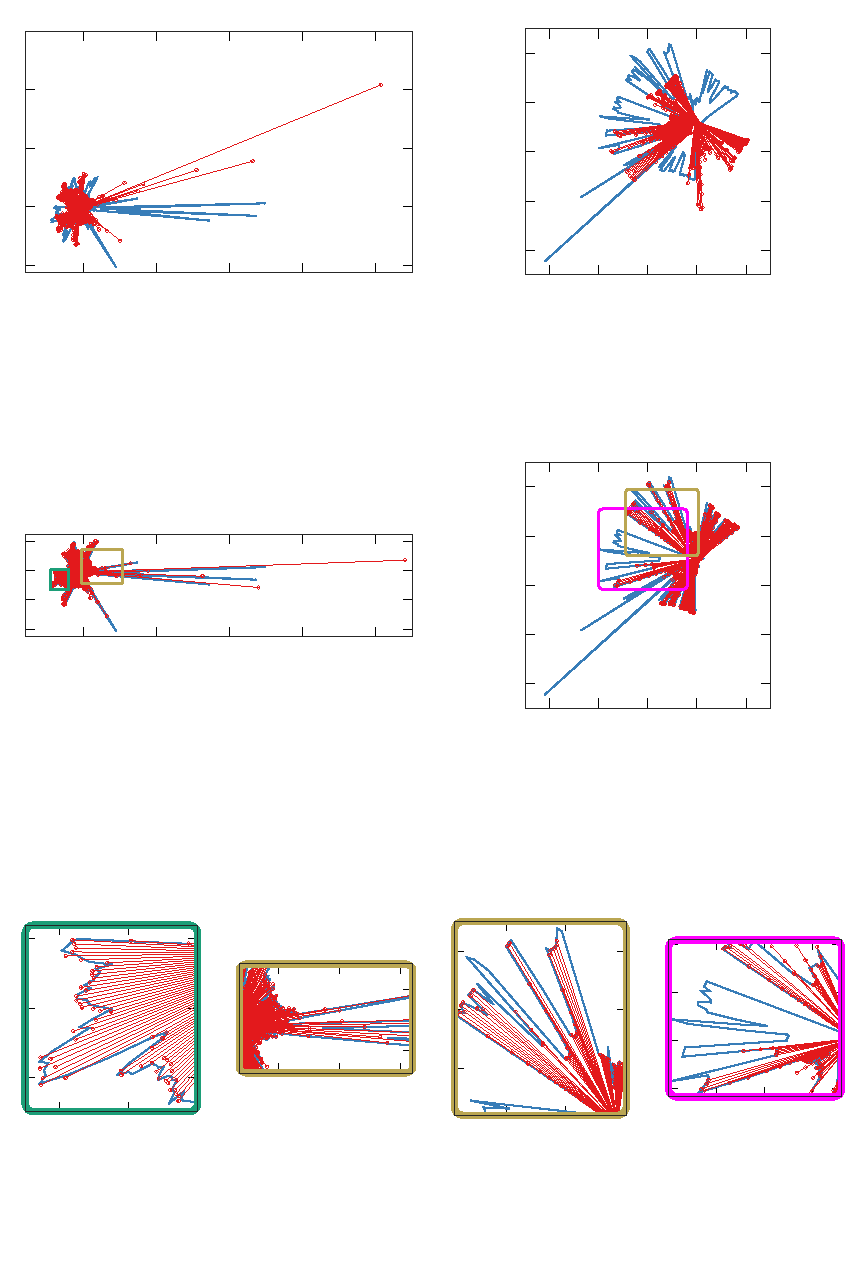
\includegraphics{./figures/parts/02/chapters/05/sections/04/from_video}}%
    \gplfronttext
  \end{picture}%
\endgroup
